%!TeX root=../tese.tex
%("dica" para o editor de texto: este arquivo é parte de um documento maior)
% para saber mais: https://tex.stackexchange.com/q/78101/183146

\chapter{Benchmarks}
\label{chap:benchmarks}

\section{Metodologia}
Os algoritmos foram implementados na linguagem C++ usando apenas as bibliotecas
padrão e a STL. Todos os programas foram compilados com a versão 7.4.0 do
compilador g++, num computador que possui um processador Intel Core i5-8250U
com clock base de 1.60GHz e turbo boost até 3.40GHz em uma única thread. As medições
de tempo foram feitas com o \texttt{steady\_clock} da biblioteca \texttt{<chrono>},
utilizando uma precisão de nanosegundos, tomando o devido cuidado de cronometrar apenas
as partes relevantes do código. Todos os programas foram compilados com a flag
\texttt{-O2} para permitir otimizações por parte do compilador.

Para cada algoritmo apresentado neste trabalho, foram medidos os tempos de execução tanto
da parte de preprocessamento quanto da parte de consultas, separadamente. Cada teste
também foi realizado com árvores lineares, binárias e quaternárias para evidenciar 
possíveis diferenças de performance de acordo com o formato da árvore.

Todas as árvores geradas para fins destes testes são completas (portanto balanceadas) 
e seus tamanhos variaram entre 150K e 21.6M. Tanto os testes de preprocessamento quanto
os de consultas foram executados dez vezes com cada tamanho de árvore para tomar então
suas médias como resultado. 

Os testes de preprocessamento consistem em um programa que cria uma árvore completa
com a quantidade de nós e o fator de ramificação desejados e então cria um objeto da
classe associada ao algoritmo a ser testado, o que equivale à fase de preprocessar a
árvore de entrada. Já os testes de consultas consistem em um programa que cria também
uma árvore completa com os mesmos parâmetros e então executam um conjunto de 10M de
consultas gerado previamente. Estes arquivos foram gerados aleatoriamente de forma que
toda consulta seja composta por um nó válido (entre 0 e $N-1$) onde $N$ é o tamanho do
experimento e uma profundidade válida (entre 0 e \textit{profundidade(u)}, onde $u$ é
o nó da consulta.

\section{Análise dos resultados}
As árvores que surgiriam em aplicações reais possivelmente não seriam exatamente como
as árvores aqui testadas, que são todas completas, porém ainda podemos ter uma boa
noção de como as diferentes implementações se comportam no pior caso possível e em casos
mais favoráveis.

\subsection{Preprocessamento}

\subsubsection{Árvores lineares}
A primeira coisa a ser notada é que, para árvores lineares, o Algoritmo da Tabela mal
pode ser comparado com os outros, já que para este caso sua complexidade de espaço
de preprocessamento é $\bigO(n^2)$, se tornando impossível manter o programa na memória
até mesmo para o menor tamanho de árvore dos testes padrão, 150K. Apesar disso, não
achei interessante diminuir as árvores para que os testes não se tornassem facilmente
influenciáveis por fatores do sistema como trocas de contexto, por exemplo. Como
evidenciado na figura~\ref{fig:proclinearsmall}, o Algoritmo da Tabela tem desempenho
muito pior do que todos os outros até mesmo para os testes reduzidos, o que me dá
segurança para afirmar, juntamente com sua análise de complexidade, que ele também
levaria muito mais tempo para completar os testes padrão.

\begin{figure}
  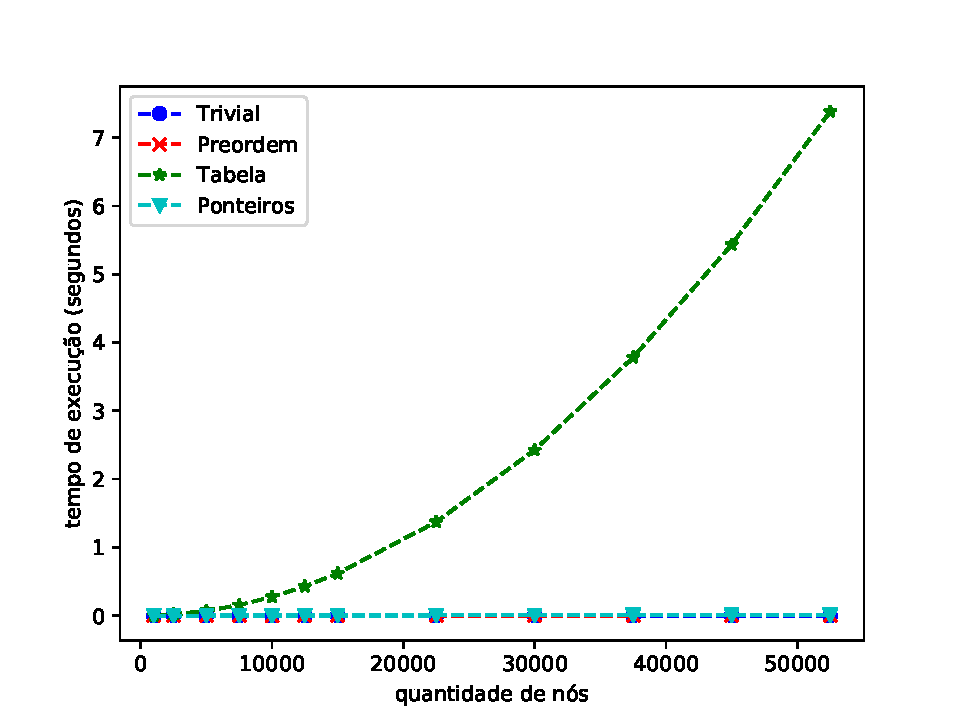
\includegraphics[scale=0.75]{preprocess_linear_smaller.pdf}
  \caption{Resultados para o preprocessamento de árvores lineares com uma versão
  reduzida dos testes.}
  \label{fig:proclinearsmall}
\end{figure}

Seguindo para a bateria normal de testes, o algoritmo Trivial, como esperado, é
definitivamente o mais rápido, se mantendo essencialmente constante a menos de pequenas
variações, seguido pelo algoritmo da Preordem que leva uma vantagem grande sobre o
algoritmo dos Ponteiros já que este é $\bigO(n \log n)$ enquanto o primeiro é $\bigO(n)$.

\begin{figure}
  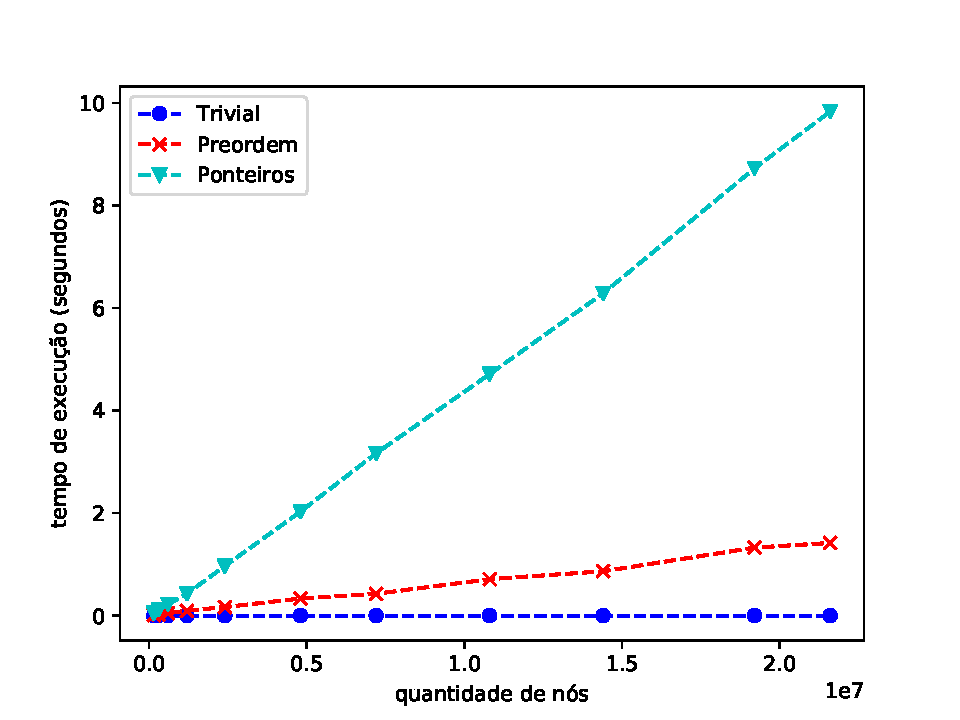
\includegraphics[scale=0.75]{preprocess_linear.pdf}
  \caption{Resultados para o preprocessamento de árvores lineares com os testes padrão.}
\end{figure}

\newpage

\subsubsection{Árvores binárias}
Para estes testes estamos considerando árvores binárias completas com profundidade
esperada $\log_2 n$ onde $n$ é o tamanho do teste, o que torna possível por exemplo
rodar o Algoritmo da Tabela para todos os tamanhos já que sua complexidade de espaço
se torna $\bigO(n \log n)$, sendo comparável com o Algoritmo dos Ponteiros, que ainda
se mostra mais eficiente pela constante menor. O Algoritmo da Preordem se tornou ainda
mais rápido se comparado aos testes com árvores lineares apesar de sua complexidade não
depender da profundidade da árvore, provavelmente por serem necessárias menos alocações
de memória.

\begin{figure}
  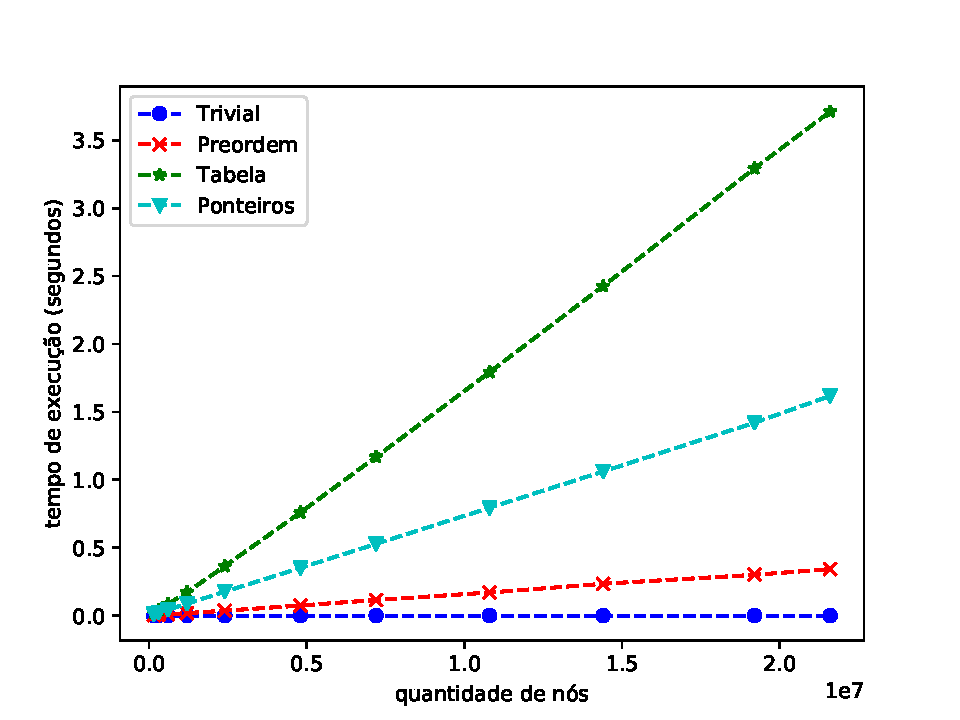
\includegraphics[scale=0.75]{preprocess_binary_new.pdf}
  \caption{Resultados para o preprocessamento de árvores binárias.}
\end{figure}

\subsubsection{Árvores quaternárias}
Para estas árvores é interessante notar que o desempenho dos algoritmos da Tabela e dos
Ponteiros foram melhores do que para árvores binárias e isso se deve à relação entre
suas complexidades de tempo e o fator de ramificação da árvore. O Algoritmo dos Ponteiros
se manteve estável já que sua complexidade não depende da forma da árvore, o que o
torna pouco adaptável ao formato da entrada.

\begin{figure}[H]
  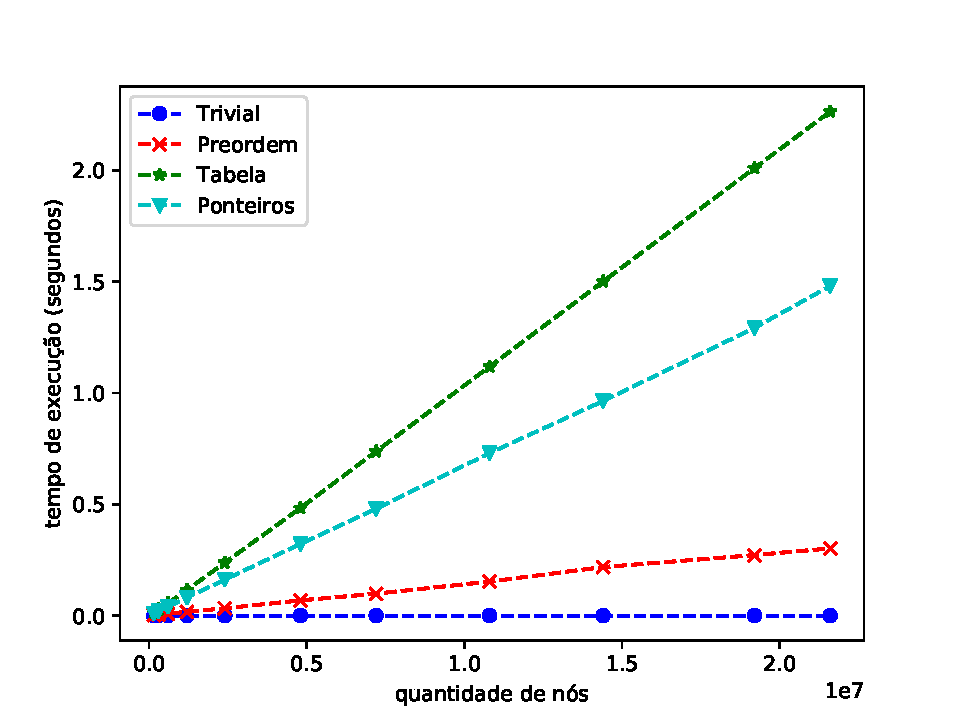
\includegraphics[scale=0.75]{preprocess_4ary_new.pdf}
  \caption{Resultados para o preprocessamento de árvores quaternárias.}
\end{figure}

\subsection{Consultas}

\subsubsection{Árvores lineares}
Aqui, assim como no caso dos testes de preprocessamento, não são todos os algoritmos
que conseguiram passar pela bateria de testes padrão. O Algoritmo da Tabela segue com
sua limitação de memória, porém agora o Algoritmo Trivial fica bastante lento, chegando
perto dos 20 segundos para 1K consultas no maior tamanho de árvore e a
metodologia escolhida para os testes de consulta fez com que o Algoritmo dos Ponteiros
também não conseguisse ter memória suficiente já que o arquivo de teste era carregado
simultaneamente na memória do computador. Todavia, como espera-se que o tempo necessário
para responder uma quantidade $m$ de consultas seja uma função linear em $m$, é possível
obter resultados ainda significativos a partir do teste reduzido.

\begin{figure}[H]
  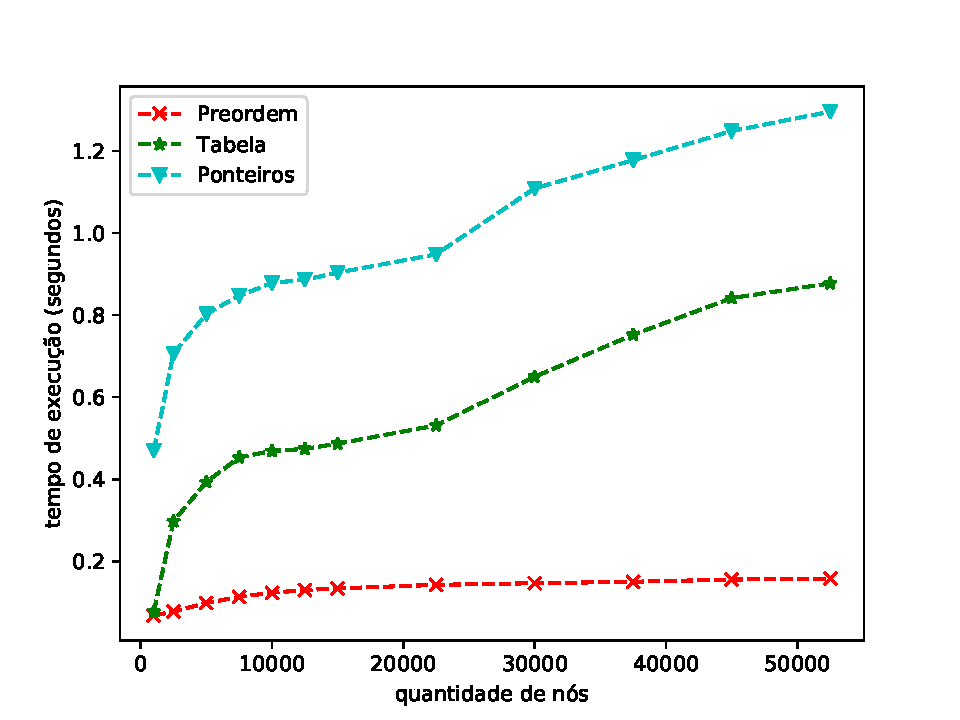
\includegraphics[scale=0.75]{query_linear_smaller.pdf}
  \caption[Resultados para o teste reduzido de consultas em árvores lineares.]
  {\textbf{Resultados para o teste reduzido de consultas em árvores lineares.}
  Para efeito de comparação, o tempo esperado para o Algoritmo Trivial executar 10M
  consultas para o maior tamanho de árvore deste teste é de aproximadamente 7 minutos
  e por isso nem está no gráfico.}
\end{figure}

\subsubsection{Árvores binárias}
Os testes de consultas em árvores binárias evidenciaram a grande melhora que o Algoritmo
Trivial consegue obter, já que, ao limitar a profundidade das árvores testadas em
$\bigO(\log_2 n)$, cada uma de suas consultas também é realizada em tempo logarítmico.
Já os algoritmos da Preordem e dos Ponteiros têm performances semelhantes, porém, 
o segundo leva a melhor. O Algoritmo da Tabela, como esperado, se mantém constante
e extremamente rápido.

Vale lembrar também que esses resultados correspondem à realização de 10 milhões de
consultas, ou seja, até mesmo o Algoritmo Trivial é capaz de realizar uma única consulta
em tempos quase insignificantes (na ordem de $9.25\mathrm{e}{-07}$ segundos).

\begin{figure}[H]
  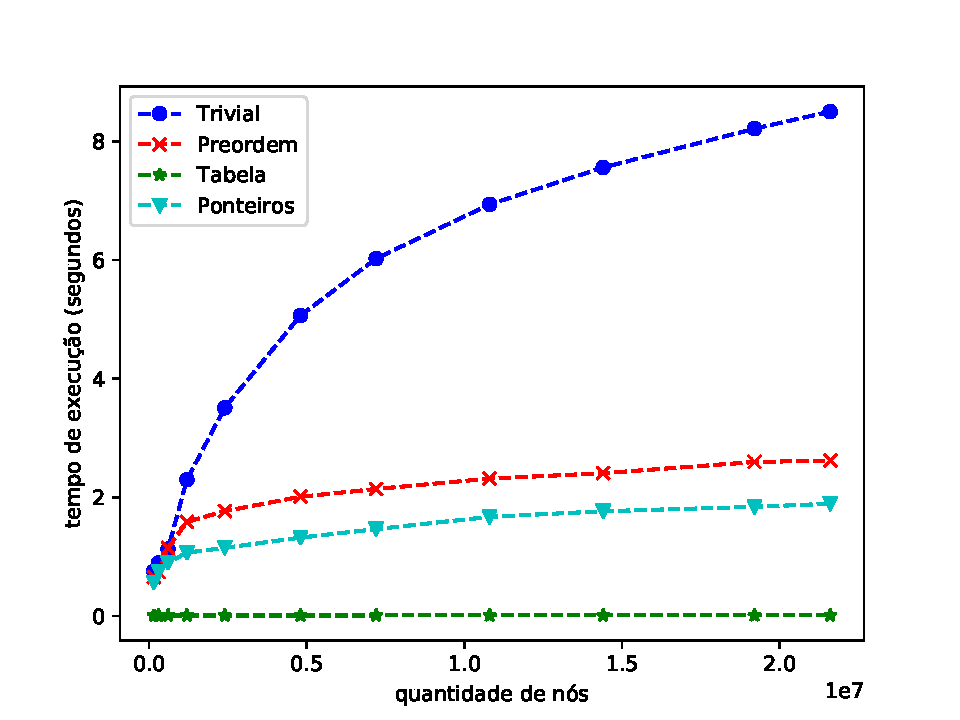
\includegraphics[scale=0.75]{query_binary_new.pdf}
  \caption{Resultados para as consultas em árvores binárias.}
\end{figure}

\subsubsection{Árvores quaternárias}
Aqui, o Algoritmo Trivial se torna ainda mais eficiente devido à limitação da
profundidade das árvores em $\bigO(\log_4 n)$, ficando muito mais próximo dos seus
concorrentes e ficando abaixo de de 5 segundos para 10 milhões de consultas no maior
tamanho de árvore testado. Os algoritmos da Preordem e dos Ponteiros se mantiveram
praticamente iguais ao teste anterior, provavelmente devido às suas constantes já serem
suficientemente pequenas para árvores binárias.

\begin{figure}[H]
  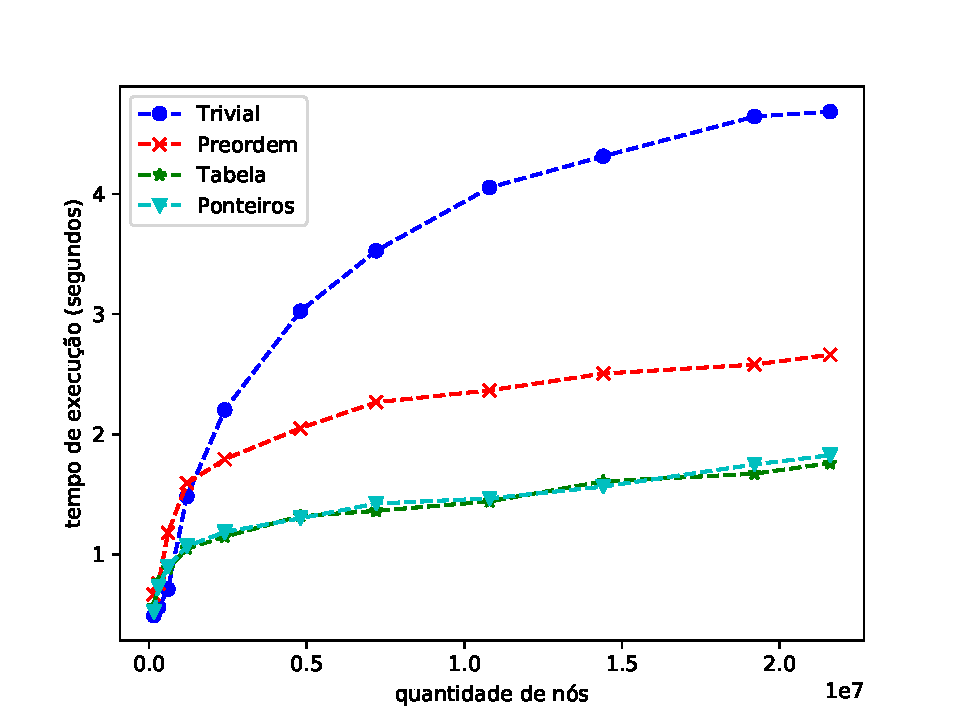
\includegraphics[scale=0.75]{query_4ary_new.pdf}
  \caption{Resultados para as consultas em árvores quaternárias.}
\end{figure}

\section{Uso de memória}

Uma parte muito importante da comparação dos algoritmos implementados é analisar seu
consumo de memória, já que além de ser um fator proibitivo para muitos computadores
pessoais também pode influenciar a performance de um algoritmo caso fique no limite
da memória disponível. Os valores presentes nas tabelas abaixo foram obtidos através
do programa \texttt{/usr/bin/time -v} do Linux, exceto para o Algoritmo da Tabela
no caso das árvores lineares.

\subsection{Árvores lineares}
Observando a quantidade necessária de memória para preprocessar árvores lineares com
cada um dos algoritmos pode-se ver porque o Algoritmo da Tabela é inviável para este
caso do problema, já que atingiria quantidades absurdas devido à sua complexidade
quadrática. O Algoritmo dos Ponteiros apresenta uma quantidade de memória utilizada
maior que o Algoritmo da Preordem, como esperado, já que o primeiro tem uma constante
que multiplica sua complexidade.

\begin{table}[H]
  \begin{tabular}{|l|l|l|l|l|}
  \hline
  \textbf{Nós}            & \textbf{Trivial} & \textbf{Tabela *} & \textbf{Ponteiros} & \textbf{Preordem} \\ \hline
  \textbf{150K}  & 0.017            & 44                & 0.034              & 0.028             \\ \hline
  \textbf{300K}  & 0.031            & 176               & 0.066              & 0.053             \\ \hline
  \textbf{600K}  & 0.059            & 704               & 0.129              & 0.104             \\ \hline
  \textbf{1.2M}  & 0.11             & 2816              & 0.256              & 0.206             \\ \hline
  \textbf{2.4M}  & 0.22             & 11264             & 0.546              & 0.410             \\ \hline
  \textbf{4.8M}  & 0.45             & 45056             & 1.09               & 0.818             \\ \hline
  \textbf{7.2M}  & 0.67             & 101376            & 1.63               & 1.12              \\ \hline
  \textbf{9.6M}  & 0.90             & 228096            & 2.17               & 1.63              \\ \hline
  \textbf{10.8M} & 1.01             & 513216            & 2.44               & 1.75              \\ \hline
  \textbf{14.4M} & 1.35             & 1154736           & 3.26               & 2.25              \\ \hline
  \textbf{19.2M} & 1.80             & 2598156           & 4.35               & 3.26              \\ \hline
  \textbf{21.6M} & 2.02             & 3259126           & 4.89               & 3.50              \\ \hline
  \end{tabular}
  \caption[Uso de memória (em GB) de cada algoritmo para preprocessar árvores lineares.]
  {\textbf{Uso de memória (em GB) de cada algoritmo para preprocessar árvores lineares.}
   Os valores do Algoritmo da Tabela foram estimados, já que não é possível rodá-lo
   para estes tamanhos. Além disso, é importante notar que está incluso nestes valores
   a árvore em si, já que mesmo o Algoritmo Trivial, que não realiza preprocessamento
   nenhum, ainda precisa acessar a estrutura da árvore.}
  \end{table}

\subsection{Árvores binárias}
Com os testes restringidos a árvores binárias, o Algoritmo da Tabela consegue realizar
o preprocessamento sem estourar a memória da máquina utilizada, mas ainda apresenta uma
quantidade significativamente maior que os outros algoritmos, o que pode se tornar
um problema eventualmente para casos extremos. Além disso, todos os outros algoritmos
também apresentaram um uso reduzido de memória, como esperado.

\begin{table}[H]
  \begin{tabular}{|l|l|l|l|l|}
  \hline
  \textbf{Nós}   & \textbf{Trivial} & \textbf{Tabela} & \textbf{Ponteiros} & \textbf{Preordem} \\ \hline
  \textbf{150K}  & 0.014            & 0.029             & 0.029              & 0.016             \\ \hline
  \textbf{300K}  & 0.026            & 0.057             & 0.042              & 0.030             \\ \hline
  \textbf{600K}  & 0.050            & 0.115             & 0.082              & 0.057             \\ \hline
  \textbf{1.2M}  & 0.096            & 0.232             & 0.162              & 0.112             \\ \hline
  \textbf{2.4M}  & 0.190            & 0.467             & 0.322              & 0.221             \\ \hline
  \textbf{4.8M}  & 0.377            & 0.945             & 0.640              & 0.439             \\ \hline
  \textbf{7.2M}  & 0.565            & 1.45              & 0.959              & 0.670             \\ \hline
  \textbf{9.6M}  & 0.753            & 1.95              & 1.27               & 0.877             \\ \hline
  \textbf{10.8M} & 0.846            & 2.21              & 1.43               & 0.989             \\ \hline
  \textbf{14.4M} & 1.12             & 2.97              & 1.91               & 1.33              \\ \hline
  \textbf{19.2M} & 1.50             & 3.98              & 2.55               & 1.75              \\ \hline
  \textbf{21.6M} & 1.69             & 4.48              & 2.87               & 1.97              \\ \hline
  \end{tabular}
  \caption[Uso de memória (em GB) de cada algoritmo para preprocessar árvores binárias.]
  {\textbf{Uso de memória (em GB) de cada algoritmo para preprocessar árvores binárias.}
   Note que está incluso nestes valores a árvore em si, já que mesmo o Algoritmo Trivial,
   que não realiza preprocessamento nenhum, ainda precisa acessar a estrutura da árvore.}
  \end{table}

\subsection{Árvores quaternárias}
Nestes testes, é possível observar uma pequena redução da memória utilizada pelos
algoritmos Trivial e da Preordem, apesar de seu preprocessamento não depender do fator
de ramificação da árvore e o Algoritmo dos Ponteiros viu um ganho também pequeno, já
que a mudança de $n \log_2(\log_2 n)$ para $n \log_4(\log_4 n)$ não é tão expressiva.
Isto indica que, para fatores de ramificação maiores ainda, a quantidade de memória
utilizada pelos algoritmos deve se estabilizar não muito longe dos valores desta tabela.

\begin{table}[H]
  \begin{tabular}{|l|l|l|l|l|}
  \hline
  \textbf{Nós}   & \textbf{Trivial} & \textbf{Tabela} & \textbf{Ponteiros} & \textbf{Preordem} \\ \hline
  \textbf{150K}  & 0.014            & 0.024             & 0.022              & 0.016             \\ \hline
  \textbf{300K}  & 0.025            & 0.046             & 0.041              & 0.029             \\ \hline
  \textbf{600K}  & 0.047            & 0.093             & 0.080              & 0.055             \\ \hline
  \textbf{1.2M}  & 0.092            & 0.189             & 0.157              & 0.109             \\ \hline
  \textbf{2.4M}  & 0.181            & 0.381             & 0.312              & 0.214             \\ \hline
  \textbf{4.8M}  & 0.354            & 0.766             & 0.622              & 0.429             \\ \hline
  \textbf{7.2M}  & 0.537            & 1.15              & 0.931              & 0.632             \\ \hline
  \textbf{9.6M}  & 0.715            & 1.53              & 1.24               & 0.847             \\ \hline
  \textbf{10.8M} & 0.804            & 1.72              & 1.39               & 0.966             \\ \hline
  \textbf{14.4M} & 1.07             & 2.30              & 1.85               & 1.31              \\ \hline
  \textbf{19.2M} & 1.42             & 3.07              & 2.47               & 1.69              \\ \hline
  \textbf{21.6M} & 1.60             & 3.45              & 2.78               & 1.87              \\ \hline
  \end{tabular}
  \caption[Uso de memória (em GB) de cada algoritmo para preprocessar árvores quaternárias.]
  {\textbf{Uso de memória (em GB) de cada algoritmo para preprocessar árvores quaternárias.}
   Note que está incluso nestes valores a árvore em si, já que mesmo o Algoritmo Trivial,
   que não realiza preprocessamento nenhum, ainda precisa acessar a estrutura da árvore.}
  \end{table}

\section{Conclusões e trabalho futuro}
Analisando os resultados fica evidente o quão importante é conhecer a tanto a aplicação
em questão quanto os recursos disponíveis, já que cada algoritmo tem méritos e defeitos
que dependem do formato das árvores. O Algoritmo da Tabela é uma ótima escolha para
aplicações em que a quantidade de consultas pesa muito mais do que o tempo de
preprocessamento, já que este abre mão de performance \textit{a priori} para responder
as consultas o mais rápido possível; entretanto, também possui um custo proibitivo de
memória conforme o fator de ramificação diminui, que pode torná-lo inviável até mesmo
para \textit{workstations} com grandes quantidades de memória. O Trivial se torna mais
viável conforme o fator de ramificação aumenta e tem custo zero de memória e tempo de
preprocessamento, porém não lida muito bem com seu pior caso de árvores lineares,
levando tempos que tornariam qualquer aplicação ineficaz conforme o tamanho das árvores
aumentam. Tanto o Algoritmo dos Ponteiros quanto o Algoritmo da Preordem trazem soluções
elegantes com boas complexidades tanto para o preprocessamento quanto para as consultas,
porém de mais difícil compreensão; o primeiro leva a melhor nas consultas (exceto no caso
de árvores lineares) ao passo que o segundo conta com o melhor preprocessamento de
todos (a menos do Trivial, que não faz nada).

Numa continuação deste trabalho, seria interessante expandir o estudo para o caso do
Problema do Ancestral de Nível \textbf{dinâmico}, no qual a árvore do problema pode ser
modificada em tempo de execução. Logo de cara é fácil perceber que o Algoritmo Trivial
funcionaria sem nenhuma adaptação, enquanto os outros teriam que gastar algum tempo
reprocessando a árvore, o que leva a mais discussões interessantes. Além disso, seria
bom testar os algoritmos com árvores não completas, talvez obtendo comparações mais
condizentes com casos reais das aplicações do problema.